\pagestyle{empty}


\begin{frame}{One iteration of the simplex algorithm}

 \begin{tabbing}
    Start with feasible basis $B$ \\[1ex]
    {\tt while} \= $B$ is not optimal \\ [.7ex]
    \> Let $i \in B$ be index with $\lambda_i<0$ \\
    \> Compute  $d \in \setR^n$ with $a_j^T d = 0, \, j \in B \setminus\{i\}$
    and $a_i^T d = -1$ \\ 
    \> Determine $K = \{ k \colon 1 \leq k \leq m, \, a_k^Td >0\}$\\[.7ex]  
    \> {\tt if} \= $K = \emptyset$ \\   
    \> \> \emph{assert LP unbounded} \\
    \> {\tt else} \\
    \> \> Let $k \in K$ index where 
    $
    \displaystyle \min_{k \in K} (b_k - a_k^Tx^*)/a_k^Td
    $
    is attained \\ %(with  $x^* = A_B^{-1}b_B$)
    
    \> \>\emph{update} $B := B \setminus\{i\} \cup \{k\}$             
  \end{tabbing}
  
  
\end{frame}


\begin{frame}
  
\end{frame}

\begin{frame}{One iteration of the simplex algorithm}



\begin{theorem}
  \label{thr-a-4}
  One iteration of the simplex algorithm requires a total number of
  $O(m\cdot n)$ operations on rational numbers whose size is polynomial
  in the input size. 
\end{theorem}

  \begin{columns}
    \begin{column}{.5\textwidth}
      
    \end{column}
    \begin{column}{.5\textwidth}
      
    \end{column}       
  \end{columns}
\end{frame}




\begin{frame}
  

\end{frame}


\begin{frame}
  \frametitle{Smale's 18 problems for the next century }
  Problem 18: Can linear programming be solved in strongly polynomial time? 
\end{frame}

\begin{frame}
  \frametitle{Integer Programming}

  \begin{columns}
    \begin{column}{.3\textwidth}
      An \emph{integer program} is a problem of the form 
\begin{displaymath}
  \begin{array}{c}
    \max c^Tx \\
    Ax\leq b \\
    x \in \setZ^n 
  \end{array}
\end{displaymath}
with $A ∈ ℤ^{m ×n}$, $b ∈ ℤ^{m}$ and $c ∈ ℤ^n$. 
    \end{column}
    \begin{column}{.7\textwidth}
      
  \begin{center}
   \includegraphics[height=4cm]{../figures/IntProg1.pdf}
  \end{center}

    \end{column}       
  \end{columns}

\end{frame}



\begin{frame}{Complexity of integer programming} 

  \begin{theorem}
    The integer feasibility problem is NP-complete. 
  \end{theorem}
  
\end{frame}



\begin{frame}
  
\end{frame}

\begin{frame}{The LP-relaxation}
\begin{theorem}
  \label{thr:14}
  Suppose that   $x^*$ is an  optimal solution of the  
  \emph{linear programming 
    relaxation} $\max\{c^Tx \colon Ax\leq b, x ∈ ℝ^n\}$
  Then $c^T x^* ≥ c^T x_I$, for each integer feasible solution. 
\end{theorem}



\begin{theorem}
  \label{thr:14}
  Suppose that   $x^*$ is an integral  optimal solution of the  
  linear programming 
  relaxation $\max\{c^Tx \colon Ax\leq b, x ∈ ℝ^n\}$, i.e., $x^* \in
  \setZ^n$, then $x^*$ is also an optimal solution of the integer
  programming problem $\max\{c^Tx \colon Ax\leq b, \, x \in \setZ^n\}$
\end{theorem}


   \begin{columns}
    \begin{column}{.5\textwidth}
      
    \end{column}
    \begin{column}{.5\textwidth}
      
    \end{column}       
  \end{columns}
\end{frame}





\begin{frame}{Undirected graphs -- Matchings} 


   \begin{columns}
    \begin{column}{.5\textwidth}
      
\begin{definition} 
  An \emph{undirected graph} is a tuple $G = (V,E)$

  \medskip 
  $V$ is 
  finite set of  \emph{vertices}

  \medskip 
  $E\subseteq\binom{V}{2}$ is 
  set of \emph{edges} of $G$.

  \medskip 
  \emph{Matching}: 
  $M\subseteq E$ such that for all $e_1\neq e_2\in M$ one has $e_1\cap e_2 = \emptyset$. 
\end{definition}
    \end{column}
    \begin{column}{.5\textwidth}
      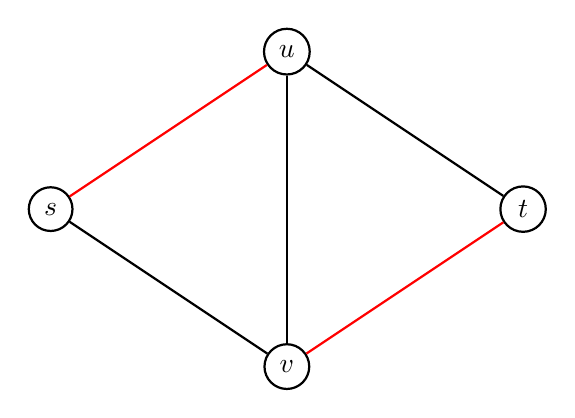
\begin{tikzpicture}[style=thick]
%\draw[help lines] (0,0) grid (2,5);
\tikzstyle{vertex}=[draw,shape=circle]
\tikzstyle{edge} = [draw,thick,-]
\tikzstyle{weight} = [font=\small];

\draw (0,0) node[vertex] (s) {$s$};
\draw (3,2) node[vertex] (u) {$u$};
\draw (3,-2) node[vertex] (v) {$v$};
\draw (6,0) node[vertex] (t) {$t$};

\draw[red]  (s) --  (u);
\draw        (s) --  (v);
\draw  (u) -- (v);
\draw (u) -- (t);
\draw [red] (v) -- (t);
\end{tikzpicture}
    \end{column}       
  \end{columns}
\end{frame}




\begin{frame}{$δ(v)$}

  
For a vertex $v \in V$, the set $\delta(v) = \{e \in E \colon v \in e\}$ denotes
the \emph{incident} edges to $v$. 
  
\end{frame}


\begin{frame}{Modeling max-weight matching as integer program} 


  \begin{equation*}
  \label{eq:45}
  \begin{array}{c}\displaystyle 
    \max \sum_{e \in E} w(e) x(e) \\
    \displaystyle 
    v \in V: \, \sum_{e \in \delta(v)} x(e)\leq1 \\
    \displaystyle 
    e \in E:\,  x(e)  \geq0 \\
    \displaystyle 
    x \in \setZ^{|E|}.
  \end{array}
\end{equation*}

   \begin{columns}
    \begin{column}{.5\textwidth}
      
    \end{column}
    \begin{column}{.5\textwidth}
      
    \end{column}       
  \end{columns}
\end{frame}



\begin{frame}{Example} 
  
\end{frame}



\begin{frame}{Integral polyhedra}

  




   \begin{columns}
    \begin{column}{.5\textwidth}
      \begin{definition}
  \label{def:12}  
  A rational polyhedron   is called \emph{integral} 
  if  each nonempty face of $P$ contains an integer vector. 
\end{definition}
    \end{column}
    \begin{column}{.5\textwidth}
      
    \end{column}       
  \end{columns}
\end{frame}





\begin{frame}{Simplex on polyhedra whose vertices are integral}

  
\begin{lemma}
  \label{lem:9}
  Let $P = \{ x \in \setR^n \colon Ax\leq b\}$ be an integral polyhedron with $A
  \in \setR^{m\times n}$ full-column rank. If the linear program 
  \begin{equation}
    \label{eq:44}
    \max\{c^Tx \colon x \in \setR^n, \, Ax\leq b\}
  \end{equation}
  is feasible and bounded, then the simplex method computes an optimal
  integral solution to the linear program. 
\end{lemma}


   \begin{columns}
    \begin{column}{.5\textwidth}
      
    \end{column}
    \begin{column}{.5\textwidth}
      
    \end{column}       
  \end{columns}
\end{frame}




\begin{frame}{The study of integral polyhedra}

  \begin{lemma}
  \label{po:lem:6}
  Let $A\in \setZ^{n\times n}$ be an integral and invertible matrix. One has
  $A^{-1}b \in \setZ^n$ for each $b \in \setZ^n$ if and only if $\det(A)=\pm 1$.
\end{lemma}



   \begin{columns}
    \begin{column}{.5\textwidth}
      
    \end{column}
    \begin{column}{.5\textwidth}
      
    \end{column}       
  \end{columns}
\end{frame}




\begin{frame}


   \begin{columns}
    \begin{column}{.5\textwidth}
      
    \end{column}
    \begin{column}{.5\textwidth}
      
    \end{column}       
  \end{columns}
\end{frame}





\begin{frame}


   \begin{columns}
    \begin{column}{.5\textwidth}
      
    \end{column}
    \begin{column}{.5\textwidth}
      
    \end{column}       
  \end{columns}
\end{frame}





\begin{frame}


   \begin{columns}
    \begin{column}{.5\textwidth}
      
    \end{column}
    \begin{column}{.5\textwidth}
      
    \end{column}       
  \end{columns}
\end{frame}




\begin{frame}


   \begin{columns}
    \begin{column}{.5\textwidth}
      
    \end{column}
    \begin{column}{.5\textwidth}
      
    \end{column}       
  \end{columns}
\end{frame}




\begin{frame}


   \begin{columns}
    \begin{column}{.5\textwidth}
      
    \end{column}
    \begin{column}{.5\textwidth}
      
    \end{column}       
  \end{columns}
\end{frame}





\begin{frame}


   \begin{columns}
    \begin{column}{.5\textwidth}
      
    \end{column}
    \begin{column}{.5\textwidth}
      
    \end{column}       
  \end{columns}
\end{frame}





\begin{frame}


   \begin{columns}
    \begin{column}{.5\textwidth}
      
    \end{column}
    \begin{column}{.5\textwidth}
      
    \end{column}       
  \end{columns}
\end{frame}




\begin{frame}


   \begin{columns}
    \begin{column}{.5\textwidth}
      
    \end{column}
    \begin{column}{.5\textwidth}
      
    \end{column}       
  \end{columns}
\end{frame}




\begin{frame}


   \begin{columns}
    \begin{column}{.5\textwidth}
      
    \end{column}
    \begin{column}{.5\textwidth}
      
    \end{column}       
  \end{columns}
\end{frame}





\begin{frame}


   \begin{columns}
    \begin{column}{.5\textwidth}
      
    \end{column}
    \begin{column}{.5\textwidth}
      
    \end{column}       
  \end{columns}
\end{frame}





\begin{frame}


   \begin{columns}
    \begin{column}{.5\textwidth}
      
    \end{column}
    \begin{column}{.5\textwidth}
      
    \end{column}       
  \end{columns}
\end{frame}




%%% Local Variables:
%%% mode: LaTeX
%%% TeX-master: "Slides"
%%% End:


